\section{Clustering Visualization}
\label{sec:appendixb}
The full results of clustering can be seen in~\figref{fig:visualizationclusterall}.


%中插聚类可视化图
%中插聚类可视化图片

\begin{figure}[htbp]
\centering
\subfigure{
\begin{minipage}[b]{.48\linewidth}
\centering
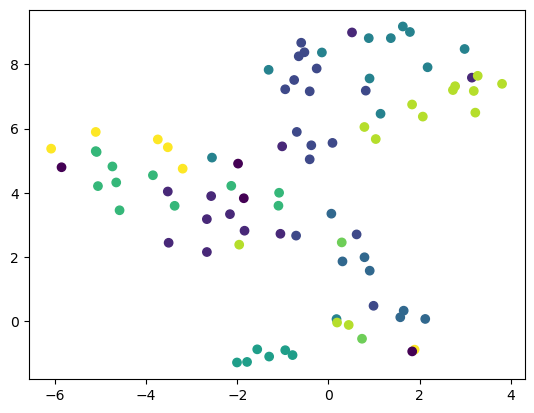
\includegraphics[scale=0.2]{cluster/shibainu_rikuchannel_sc.png}
\end{minipage}
%}
%\subfigure{
\begin{minipage}[b]{.48\linewidth}
\centering
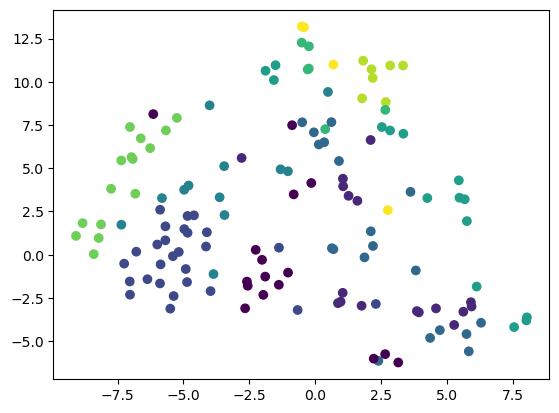
\includegraphics[scale=0.2]{cluster/ringoro_sc.png}
\end{minipage}
}
\subfigure{
\begin{minipage}[b]{.48\linewidth}
\centering
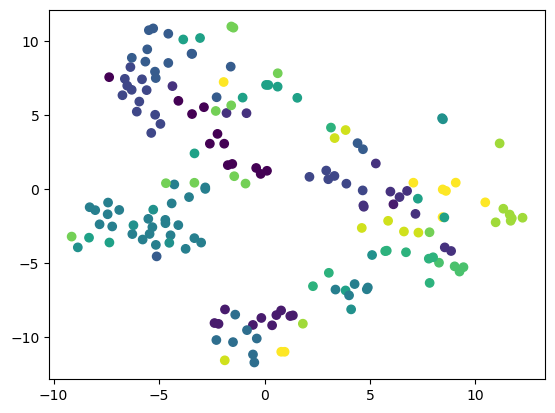
\includegraphics[scale=0.2]{cluster/hikaiti_sc.png}
\end{minipage}
%}
%\subfigure{
\begin{minipage}[b]{.48\linewidth}
\centering
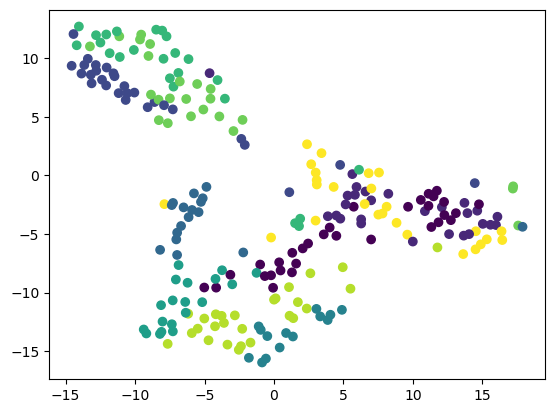
\includegraphics[scale=0.2]{cluster/jumpingmameko1822_sc.png}
\end{minipage}}

\subfigure{
\begin{minipage}[b]{.48\linewidth}
\centering
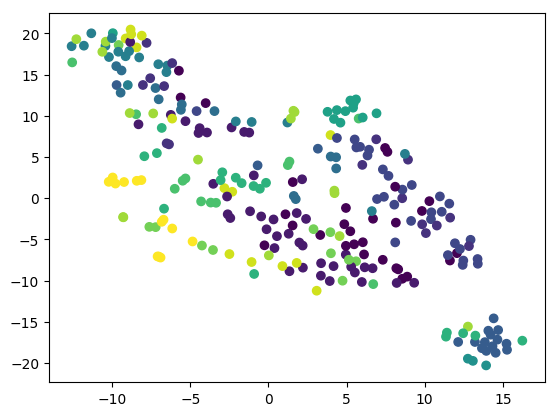
\includegraphics[scale=0.2]{cluster/shibaneko_sc.png}
\end{minipage}
%}
%\subfigure{
\begin{minipage}[b]{.48\linewidth}
\centering
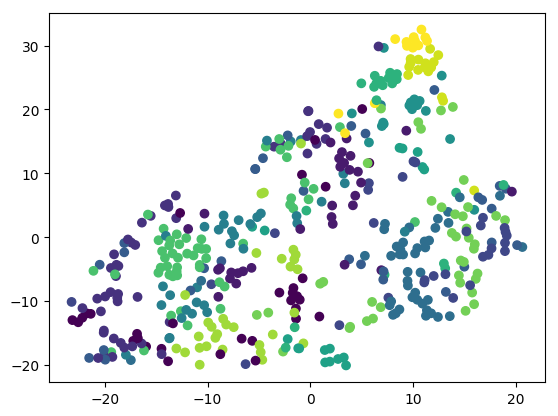
\includegraphics[scale=0.2]{cluster/shibainutakanoriawesomecha30_sc.png}
\end{minipage}
}
\subfigure{
\begin{minipage}[b]{.48\linewidth}
\centering
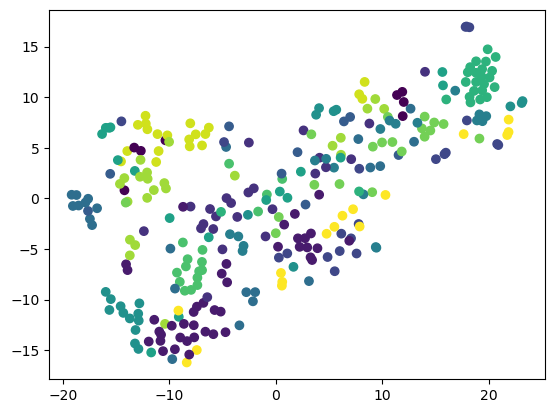
\includegraphics[scale=0.2]{cluster/MomoTenKuu_sc.png}
\end{minipage}
%}
%\subfigure{
\begin{minipage}[b]{.48\linewidth}
\centering
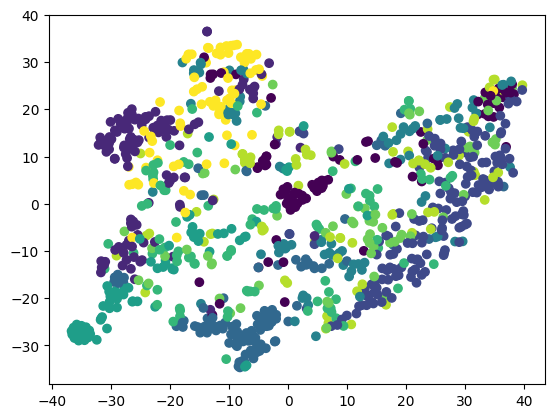
\includegraphics[scale=0.2]{cluster/mamedachamesuke_sc.png}
\end{minipage}}
\subfigure{
\begin{minipage}[b]{.48\linewidth}
\centering
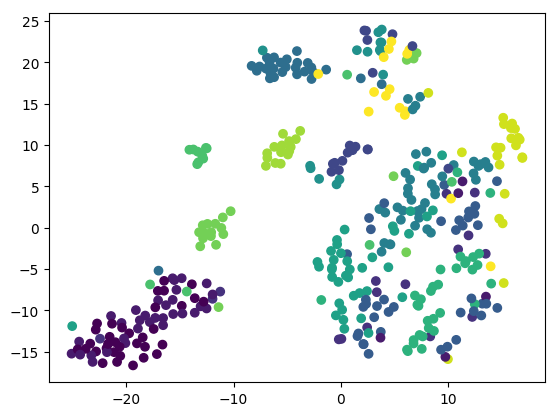
\includegraphics[scale=0.2]{cluster/ShibainuRanmaru_sc.png}
\end{minipage}
%}
%\subfigure{
\begin{minipage}[b]{.48\linewidth}
\centering
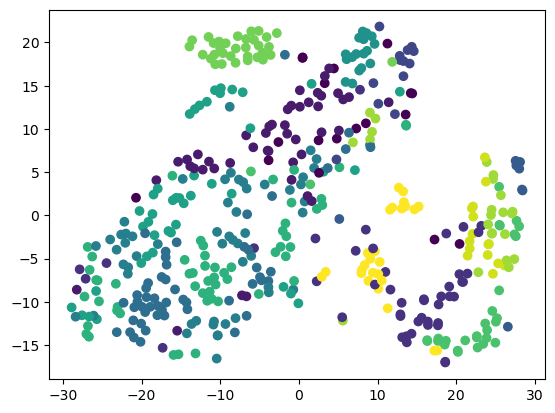
\includegraphics[scale=0.2]{cluster/shibainu-rara_sc.png}
\end{minipage}
}
\subfigure{
\begin{minipage}[b]{.48\linewidth}
\centering
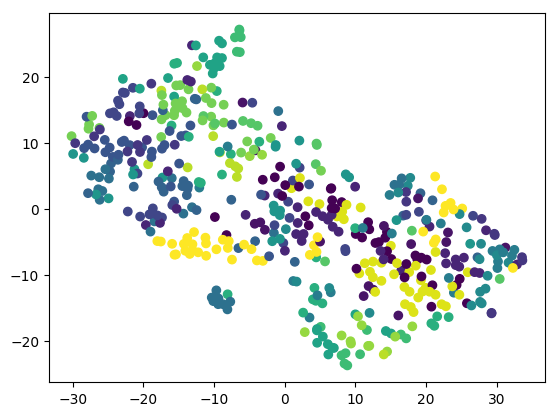
\includegraphics[scale=0.2]{cluster/ShibainuKOTETSU_sc.png}
\end{minipage}
%}
%\subfigure{
\begin{minipage}[b]{.48\linewidth}
\centering
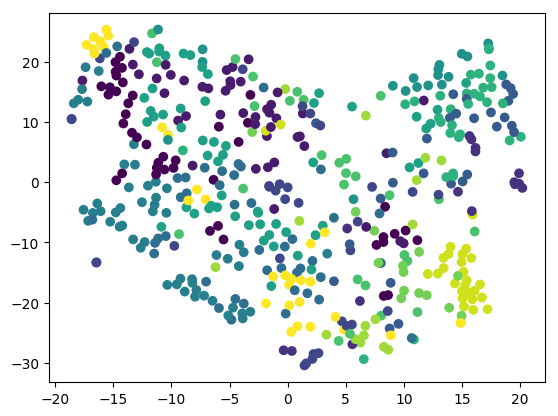
\includegraphics[scale=0.2]{cluster/shibainucatchannel7691_sc.png}
\end{minipage}
}
\subfigure{
\begin{minipage}[b]{.48\linewidth}
\centering
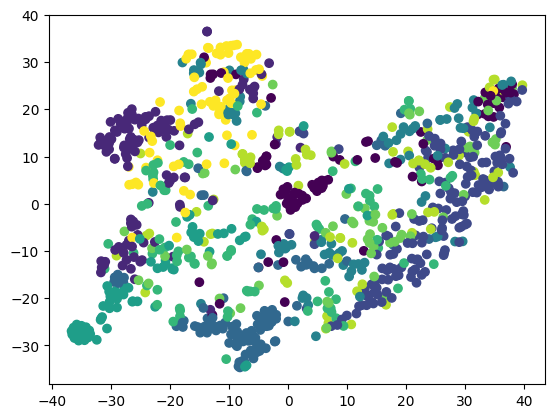
\includegraphics[scale=0.2]{cluster/mamedachamesuke_sc.png}
\end{minipage}
%}
%\subfigure{
\begin{minipage}[b]{.48\linewidth}
\centering
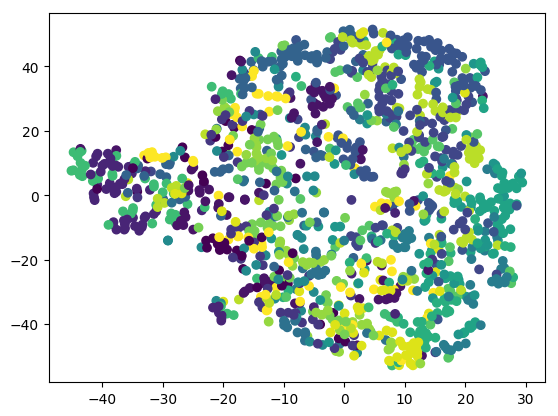
\includegraphics[scale=0.2]{cluster/user-kd8rn5jx7x_sc.png}
\end{minipage}
}
\subfigure{
\begin{minipage}[b]{.48\linewidth}
\centering
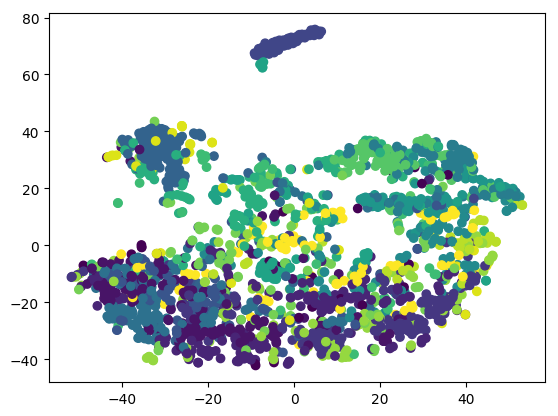
\includegraphics[scale=0.2]{cluster/shibainuTAIGA_sc.png}
\end{minipage}
%}
%\subfigure{
\begin{minipage}[b]{.48\linewidth}
\centering
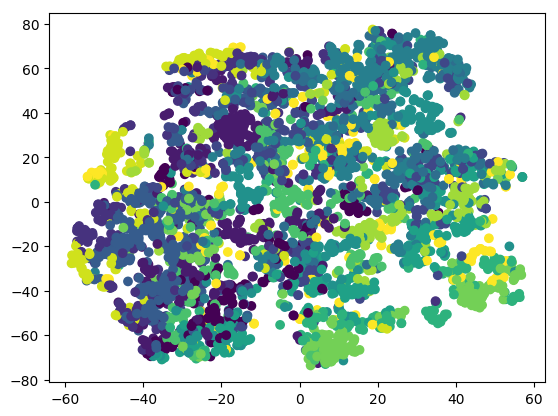
\includegraphics[scale=0.2]{cluster/ShibaInuKohachannel.png}
\end{minipage}
}
\caption{Visualization of Spectral Clustering after TSNE of 16 dogs. The dog's IDs are increasing from left to right, up to down. Phonetic symbols are assigned to different clusters. }
\label{fig:visualizationclusterall}
\end{figure}




\section{Bigram Statistical Result}
\label{sec:appendixc}

Because of the space restrictions, we don't show the detailed results in the main paper. The complete result is in~\tabref{tab:bigramfull}.

\begin{table}[th]
\centering
\small
\begin{tabular}{c|c|c|c|c|c}
\hline
\textbf{Bigram} & \textbf{Freq.} & \textbf{Co.} & \textbf{Bigram} & \textbf{Freq.} & \textbf{Co.}\\
\hline
en en & 1464 & 12 & a a & 835 & 14 \\
au au & 674 & 14 & i i & 319 & 12 \\
au en & 274 & 9 & en au & 256 & 10 \\
(w)au (w)au & 231 & 9 & \verb|^| \verb|^| & 224 & 9 \\
a en & 175 & 12 & au a & 173 & 8 \\
a au & 168 & 9 & en a & 130 & 10 \\
i en & 120 & 8 & en i & 80 & 8 \\
u: u: & 70 & 4 & (w)au en & 68 & 4 \\
a i & 55 & 9 & en (w)au & 52 & 6 \\
i au & 52 & 9 & au i & 50 & 9 \\
u u & 43 & 6 & i a & 41 & 8 \\
\verb|^| a & 29 & 7 & a \verb|^| & 28 & 6 \\
a (w)au & 25 & 7 & en u & 22 & 5 \\
(w)au a & 21 & 6 & au u: & 21 & 3 \\
u en & 20 & 4 & (w)au au & 20 & 4 \\
i \verb|^| & 20 & 6 & u: en & 17 & 2 \\
\verb|^| en & 16 & 5 & au u & 15 & 3 \\
au (w)au & 15 & 2 & \verb|^| i & 14 & 5 \\
\verb|^| au & 14 & 2 & i u: & 14 & 3 \\
u: au & 13 & 3 & en \verb|^| & 11 & 4 \\
(w)au i & 10 & 4 & u: i & 9 & 3 \\
en u: & 8 & 2 & i u & 8 & 2 \\
\verb|^| (w)au & 8 & 3 & \verb|^| u: & 8 & 2 \\
u au & 7 & 3 & k k & 6 & 2 \\
au \verb|^| & 6 & 2 & (w)au \verb|^| & 6 & 4 \\
i (w)au & 6 & 3 & u i & 6 & 2 \\
(w)au u & 6 & 2 & u: a & 6 & 1 \\
u a & 5 & 2 & u (w)au & 5 & 4 \\
a u: & 5 & 1 & u \verb|^| & 4 & 1 \\
\verb|^| u & 4 & 3 & a u & 4 & 2 \\
k a & 2 & 1 & k en & 1 & 1 \\
au k & 1 & 1 & a k & 1 & 1 \\
en k & 1 & 1 & k au & 1 & 1 \\
u: u & 1 & 1 &  &  & \\
\hline
\end{tabular}
\caption{The frequency and coverage number of 16 dogs' bigrams. Here Freq. represents for the frequency of one certain bigram, Co. represents for the numbers of dogs who have made this bigram.}
\label{tab:bigramfull}
\end{table}



\section{Activities and Scenes Covered by ShibaScript}
\label{sec:appendix_a}
44 activities and 37 scenes are covered by ShibaScript. The full statistics of them are in~\tabref{tab: activity_scene_all}.

\begin{table*}[th]\scriptsize
\begin{center}
\begin{tabular}{l p{1cm} p{1cm} p{5cm} p{5cm}}
\hline
\textbf{DogID} & \textbf{Scene Amount} & \textbf{Activity Amount} & \textbf{Scenes} & \textbf{Activities}\\
\hline
0 & 18 & 20 & bedroom, bathroom, dog bowl, cage, dining room, living room, stairs, hospital, quilt, in the arm, laun, road, other animals, shore, woods, field path, cabin & open boxes, bath, eat, walk, bark, sleep, pick sth up, roll, lick, stretch, play toys, play with dogs, sneeze, walk with a wheelchair, be held, listen to music, play with people \\ \hline

1 & 19 & 16 & cage, quilt, in the arm, by the fire, dining room, in the arm, hospital, living room, dog bowl, bedroom, road, lawn, snow, stream, field path, other animals, beach, woods, cabin & play with people, eat, be medicated, die, walk with a wheelchair, be held, be petted, sleep, bark, walk, play with dogs, wears a muzzle, run, sniff, wade in water \\\hline

2 & 16 & 12 & bedroom, living room, other animals, sofa, quilt, dog bowl, hospital, dining room, stairs, snow, road, lawn, woods, field path, other animals, cabin & walk, run, eat, bark, be held, be petted, play with people, bath, sleep, play with dogs, lick, sniff\\\hline

3 & 16 & 10 & living room, carpet, quilt, cat tree, dining room, dog bowl, by the window, lawn, other dogs, road, field path, garden, woods, shore, beach, snow & be medicated, walk with a wheelchair, walk, run, play with cats, sleep, wade in water, bow, bark, stretch\\\hline

4 & 18 & 15 & quilt, bedroom, living room, cage, heating pad, dining room, bathroom, door, cage, dog bowl, in the arm, lawn, field path, woods, terrace, stream, snow, road & eat, sleep, sprawl, play with toys, play with people, bath, walk, bask, roll, watch fireworks, be petted, run, sniff\\\hline

5 & 21 & 10 & bedroom, living room, dog bowl, bed, quilt, cage, by the window, under the bed, dining room, bathroom, other animals, lawn, beach, shore, woods, lawn, heating pad, field path, road, hill, shrine & sprawl, play with cats, eat, run, bark, be held, open boxes, bath, dig sand, climb the mountain\\\hline

6 & 14 & 13 & bedroom, carpet, dining room, bathroom, bed, quilt, door, road, sightseeing bus, other dogs, lawn, snow, cabin, garden & be petted, be vacuumed, sprawl, bark, play with people, listen to music, bath, sleep, walk, run, play with dogs, dig sand, play with toys\\\hline

7 & 15 & 12 & carpet, cage, dining room, dog bowl, bedroom, sofa, stairs, door, quilt, in the arm, snow, road, lawn, field path, other animals & walk, run, play with people, play with toys, sleep, dig the snow, sniff, eat, has its teeth be brushed, be petted, be held, hum in the sleep\\\hline

8 & 18 & 17 & bedroom, quilt, dog bowl, living room, bed, bathroom, carpet, in the arm, hospital, cage, field path, lawn, snow, road, cabin, other dogs, woods & stretch, sleep, play with people, eat, run, be petted, bath, play with dogs, squat, bark, be held, cut nails, has its teeth be brushed, play with toys, walk, wear a cone collar, pick sth up\\\hline

9 & 14 & 11 & door, quilt, living room, carpet, stairs, bed, in the arm, bathroom, cabin, road, garden, lawn, other dogs, hill & play with people, bark, walk, run, sleep, be petted, play with cats, bath, play with toys, lick, climb the mountain\\\hline

10 & 19 & 4 & bedroom, dining room, dog bowl, in the arm, quilt, bathroom, cage, other animals, hospital, woods, lawn, field path, sea, beach, garden, cabin, road, mirror & be petted, eat, sniff, sleep, walk, run, cut nails, wade in water, play with people, bath, open boxes, listen to music, surf, stretch\\\hline

11 & 13 & 13 & carpet, living room, sofa, quilt, bathroom, by the fire, bedroom, cage, dog bowl, cabin, lawn, garden, snow & play with people, be petted, sleep, bath, has its fur be brushed, walk, run, play with toys, be held, sprawl, bark, wag the tail\\\hline

12 & 17 & 14 & living room, sofa, by the window, dining room, quilt, by the fire, bedroom, cage, dog bowl, bed, on the ice, road, lawn, cabin, garden, snow & sprawl, play with people, walk, run, cut nails, blow, eat, play with toys, be petted, stretch, be held, bask, open boxes, sneeze\\\hline

13 & 13 & 15 & sofa, bedroom, living room, dining room, bathroom, vacuum, quilt, dog bowl, stairs, road, lawn, cabin, garden & be massaged, play with dogs, bath, be held, play with toys, walk, run, sleep, be petted, pee, has its fur be brushed, be held, bark, roll, sniff\\\hline

14 & 15 & 11 & bedroom, carpet, dog bowl, dining room, bed, quilt, bathroom, road, snow, lawn, other dogs, cabin, garden, field path & sleep, walk, run, play with people, be petted, play with dogs, bath, has its fur be brushed, bark, be held, eat\\\hline

15 & 15 & 11 & bedroom, living room, in the arm, quilt, dog bowl, cage, dining room, bathroom, by the window, lawn, snow, sea, beach, field path, road & eat, walk, run, sleep, bark, be petted, be held, play with cats, bath, bask, play with people\\\hline

total & 39 & 44 & bedroom, living room, dog bowl, bed, quilt, cage, by the window, under the bed, dining room, bathroom, other animals, stairs, hospital, in the arm, by the fire, cat tree, heating pad, sofa, carpet, door, lawn, beach, sea, woods, field path, road, hill, shrine, shore, cabin, stream, garden, snow, terrace, sightseeing bus, mirror, on the ice, vacuum, other dogs & open boxes, bath, eat, walk, run, bark, sleep, pick sth up, roll, lick, stretch, play with toys, play with dogs, sneeze, sniff, walk with a wheelchair, be held, be petted, listen to music, play with people, die, wears a muzzle, wade in water, be medicated, bow, bask, watch fireworks, play with cats, dig sand, climb the mountain, be vacuumed, sprawl, dig the snow, has its teeth be brushed, hum in the sleep, squat, cut nails, wear a cone collar, surf, wag the tail, blow, pee, be massaged, has its fur be brushed\\
\hline
\end{tabular} 
\end{center}
\caption{The full statistics for the scenes and activities appearing in each user. The order of the items in column ``Scene'' and ``Activities'' is not statistically significant}
\label{tab: activity_scene_all}
\end{table*}

% \tabincell{c}{Activity\\Amount}

% (TO APPENDIX)For activities, "others" includes "bow", "wag the tail", "pee", "die", "hum in the sleep", "dig the snow", "watch fireworks", "squat", "wear a muzzle", "wear a cone collar", "blow", "surf", "be vacuumed", "be medicated", "be brushed", "be massaged". For scenes, "others" includes "window", "fire", "shore", "heating pad", "hill", "stream", "vacuum", "under the bed", "cat tree", "shrine", "terrace", "bus", "mirror", "ice".

